\documentclass{article}
\usepackage{pgfplots}

\usepackage{tikz}
\usepackage{subfigure}
\usepackage{array}
\usepackage{fontspec}
\usepackage{framed,color}
\newcolumntype{C}[1]{>{\centering\arraybackslash}p{#1}}
\renewcommand{\tabcolsep}{6pt}
\renewcommand{\arraystretch}{4.7}

% no page number
\pagestyle{empty}

\usetikzlibrary{arrows,automata,pgfplots.colorbrewer,}

% Font setup for stix2: before amsmath and alike
\RequirePackage[lcgreekalpha]{stix2} % STIX2 font
\RequirePackage{microtype}[2019/11/18] % micro-typography

\pgfplotsset{
    compat=1.18,
    cycle from colormap manual style/.style={
        cycle list={
            [of colormap=Paired]
        }
    },
}

% \definecolor{global_eps}{HTML}{59a14f}
% \definecolor{local_eps}{HTML}{edc948}
% \definecolor{aleatoric}{HTML}{ff9da7}
% \definecolor{entropies}{HTML}{76b7b2}
% \definecolor{max_prob}{HTML}{f28e2b}
% \definecolor{total}{HTML}{b07aa1}
% \definecolor{epistemic}{HTML}{bab0ac}


\definecolor{darkgreen}{rgb}{0.01, 0.65, 0.18}
\definecolor{rob_blue}{rgb}{0.2, 0.72, 0.92}
\definecolor{unc_yellow}{RGB}{255, 210, 0}
\definecolor{hybrid_green}{rgb}{0.62, 0.82, 0.2}


\definecolor{global_eps}{rgb}{0.2, 0.72, 0.92}
\definecolor{local_eps}{rgb}{0.62, 0.82, 0.2}
\definecolor{aleatoric}{RGB}{232, 94, 113}
\definecolor{max_prob}{RGB}{251, 126, 58}
\definecolor{epistemic}{RGB}{130, 84, 145}
% \definecolor{margin}{RGB}{130, 84, 145}


\definecolor{groen}{RGB}{113, 168, 96}  % kleur van Pol en Soc
\definecolor{ugentgeel}{RGB}{255, 210, 0}
\colorlet{entropies}{ugentgeel!95!black}
\colorlet{margin}{hybrid_green}
\colorlet{total}{black!50}


\colorlet{epsglob}{global_eps}
\colorlet{epsloc}{epsglob!70!black}

% https://latexcolor.com
% https://tex.stackexchange.com/questions/19617/how-to-place-and-scale-tikz-pictures-in-subfigure
% https://www.reddit.com/r/LaTeX/comments/3kws7b/aligning_multiple_tikz_images_in_one_figure/

\newcommand{\maxprob}{u_{\mathrm{max}}}
\newcommand{\margin}{u_{\mathrm{marg}}}
\newcommand{\entropy}{u_H}
\newcommand{\aleatunc}{u_{a}}
\newcommand{\totunc}{u_{t}}
\newcommand{\epistunc}{u_{e}}
\newcommand{\globeps}{r_{\varepsilon,\mathrm{glob}}}
\newcommand{\loceps}{r_{\varepsilon,\mathrm{loc}}}



% \newcommand{\xmax}{275} %Australia
% \newcommand{\xmax}{399} %germa
% \newcommand{\xmax}{284} %Health
% \newcommand{\xmax}{425} %solar_bi
% \newcommand{\xmax}{128} %solar_smal
% \newcommand{\xmax}{173} %spec
\newcommand{\xmax}{258} %stud


\newcommand{\ymin}{0.70} %Australia
% \newcommand{\ymin}{0.6} %germa
% \newcommand{\ymin}{0.35} %Health
\newcommand{\ymax}{1.00}
% \newcommand{\ymax}{1.00}

\newcommand{\noiseA}{0}
\newcommand{\noiseB}{0.1}
\newcommand{\noiseC}{0.2}

\newcommand{\NtrainA}{200}
\newcommand{\NtrainB}{100}
\newcommand{\NtrainC}{50}

\begin{document}


\begin{figure}
	\centering
	\begin{tabular}{C{.06\textwidth}C{.31\textwidth}C{.31\textwidth}C{.31\textwidth}}

	\subfigure {
		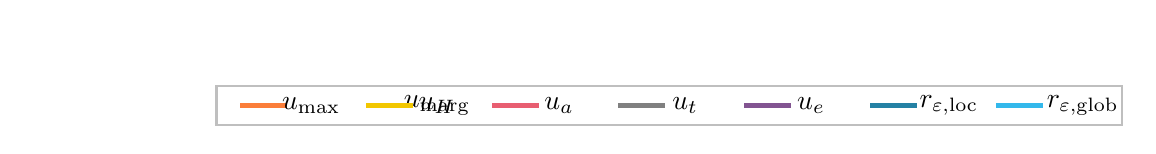
\begin{tikzpicture}
			\node[white] at (-2.15, 1) {A};
			\draw[gray!50, thick] (0,0) rectangle ++(11.5, 0.5);

			\draw[ultra thick, max_prob] (0.3, 0.25) -- (0.9, 0.25);
			\node at (1.2, 0.25) {\(\maxprob\)};

			\draw[ultra thick, margin] (1.9, 0.25) -- (2.5, 0.25);
			\node at (2.8, 0.25) {\(\margin\)};

			\draw[ultra thick, entropies] (1.9, 0.25) -- (2.5, 0.25);
			\node at (2.8, 0.25) {\(\entropy\)};

			\draw[ultra thick, aleatoric] (3.5, 0.25) -- (4.1, 0.25);
			\node at (4.35, 0.25) {\(\aleatunc\)};

			\draw[ultra thick, total] (5.1, 0.25) -- (5.7, 0.25);
			\node at (5.95, 0.25) {\(\totunc\)};

			\draw[ultra thick, epistemic] (6.7, 0.25) -- (7.3, 0.25);
			\node at (7.55, 0.25) {\(\epistunc\)};

			\draw[ultra thick, epsloc] (8.3, 0.25) -- (8.9, 0.25);
			\node at (9.3, 0.25) {\(\loceps\)};

			\draw[ultra thick, epsglob] (9.9, 0.25) -- (10.5, 0.25);
			\node at (11, 0.25) {\(\globeps\)};
		\end{tikzpicture}
		} &
	%%%%%%%%%%%%%%%%%%%%%% 1 %%%%%%%%%%%%%%%%%%%%%%%%%%%%%%%%%%%
	\subfigure {

		} &
	%%%%%%%%%%%%%%%%%%%%%% 2 %%%%%%%%%%%%%%%%%%%%%%%%%%%%%%%%%%%
	\subfigure {

		} &
	%%%%%%%%%%%%%%%%%%%%%% 3 %%%%%%%%%%%%%%%%%%%%%%%%%%%%%%%%%%%
	\subfigure {

		} \\

	\subfigure {
		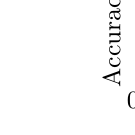
\begin{tikzpicture}
			\path[use as bounding box] (-1.5,0) rectangle (-2.5,1);
			\node[rotate=90] at (-1.40,0.9) {\small Accuracy};

			% \draw[white] (0,0) -- (0, 2);
			\draw[thick, white] (-0.665, 0) -- (0, 0);

			\node at (-0.95, 0.08) {\small \ymin};
			% \node at (-0.95, 0.70) {\small 0.8};
			% \node at (-0.95, 1.24) {\small 0.9};
			\node at (-0.95, 1.7) {\small \ymax};
		\end{tikzpicture}
		} &
	%%%%%%%%%%%%%%%%%%%%%% 1 %%%%%%%%%%%%%%%%%%%%%%%%%%%%%%%%%%%
	\subfigure {
		\begin{tikzpicture}
			\path[use as bounding box] (0,0) rectangle (2,1.2);
			\begin{axis}[
				width=0.46\textwidth,
				height=0.28\textwidth,
				cycle list/Paired,
				cycle from colormap manual style,
				ymin=\ymin, ymax=\ymax,
				xmin= 0, xmax= \xmax,
				xtick pos=left,
				xmajorticks=false,
				ymajorticks=false,
				ytick={\ymin,\ymax},
				yticklabels={\ymin,\ymax},
				% ytick={0.7,0.8,0.9,1},
				% yticklabels={0.7,0.8,0.9,1.0},
				xmajorgrids=true,
				ymajorgrids=true,
				axis line style={draw=gray!50, thick},
					]
					\addplot [no marks, very thick, max_prob] table [x={n}, y={max_prob}, col sep=comma] {files/student_port_bin_200_noise_0.0_GeFs_arc.csv};
					\addplot [no marks, very thick, margin] table [x={n}, y={margin_of_confidence}, col sep=comma] {files/student_port_bin_200_noise_0.0_GeFs_arc.csv};
					\addplot [no marks, very thick, total] table [x={n}, y={total}, col sep=comma] {files/student_port_bin_200_noise_0.0_GeFs_arc.csv};
					\addplot [no marks, very thick, aleatoric] table [x={n}, y={aleatoric}, col sep=comma] {files/student_port_bin_200_noise_0.0_GeFs_arc.csv};
					\addplot [no marks, very thick, entropies] table [x={n}, y={entropies}, col sep=comma] {files/student_port_bin_200_noise_0.0_GeFs_arc.csv};
					\addplot [no marks, very thick, epistemic] table [x={n}, y={epistemic}, col sep=comma] {files/student_port_bin_200_noise_0.0_GeFs_arc.csv};
					\addplot [no marks, very thick, epsglob] table [x={n}, y={global_eps}, col sep=comma] {files/student_port_bin_200_noise_0.0_GeFs_arc.csv};
					\addplot [no marks, very thick, epsloc] table [x={n}, y={local_eps}, col sep=comma] {files/student_port_bin_200_noise_0.0_GeFs_arc.csv};


				\end{axis}
				\node[fill=white, opacity=0.6, rounded corners, inner sep=0.1] at (2.55, 0.17) {\scriptsize \(N_{\mathrm{train}}=\NtrainA, \mathrm{DS}=\noiseA\)};
			\end{tikzpicture}
		} &
	%%%%%%%%%%%%%%%%%%%%%% 2 %%%%%%%%%%%%%%%%%%%%%%%%%%%%%%%%%%%
	\subfigure {
		\begin{tikzpicture}
			\path[use as bounding box] (0,0) rectangle (2,1.2);
			\begin{axis}[
				width=0.46\textwidth,
				height=0.28\textwidth,
				cycle list/Paired,
				cycle from colormap manual style,
				ymin=\ymin, ymax=\ymax,
				xmin= 0, xmax= \xmax,
				xtick pos=left,
				xmajorticks=false,
				ymajorticks=false,
				xmajorgrids=true,
				ymajorgrids=true,
				axis line style={draw=gray!50, thick},
					]
					\addplot [no marks, very thick, max_prob] table [x={n}, y={max_prob}, col sep=comma] {files/student_port_bin_200_noise_0.1_GeFs_arc.csv};
					\addplot [no marks, very thick, margin] table [x={n}, y={margin_of_confidence}, col sep=comma] {files/student_port_bin_200_noise_0.1_GeFs_arc.csv};
					\addplot [no marks, very thick, total] table [x={n}, y={total}, col sep=comma] {files/student_port_bin_200_noise_0.1_GeFs_arc.csv};
					\addplot [no marks, very thick, aleatoric] table [x={n}, y={aleatoric}, col sep=comma] {files/student_port_bin_200_noise_0.1_GeFs_arc.csv};
					\addplot [no marks, very thick, entropies] table [x={n}, y={entropies}, col sep=comma] {files/student_port_bin_200_noise_0.1_GeFs_arc.csv};
					\addplot [no marks, very thick, epistemic] table [x={n}, y={epistemic}, col sep=comma] {files/student_port_bin_200_noise_0.1_GeFs_arc.csv};
					\addplot [no marks, very thick, epsglob] table [x={n}, y={global_eps}, col sep=comma] {files/student_port_bin_200_noise_0.1_GeFs_arc.csv};
					\addplot [no marks, very thick, epsloc] table [x={n}, y={local_eps}, col sep=comma] {files/student_port_bin_200_noise_0.1_GeFs_arc.csv};


				\end{axis}
				\node[fill=white, opacity=0.6, rounded corners, inner sep=0.1] at (2.55, 0.17) {\scriptsize \(N_{\mathrm{train}}=\NtrainA, \mathrm{DS}=\noiseB\)};
			\end{tikzpicture}
		} &
	%%%%%%%%%%%%%%%%%%%%%% 3 %%%%%%%%%%%%%%%%%%%%%%%%%%%%%%%%%%%
	\subfigure {
	  \begin{tikzpicture}
		\path[use as bounding box] (0,0) rectangle (2,1.2);
			\begin{axis}[
				width=0.46\textwidth,
				height=0.28\textwidth,
				cycle list/Paired,
				cycle from colormap manual style,
				ymin=\ymin, ymax=\ymax,
				xmin= 0, xmax= \xmax,
				xtick pos=left,
				xmajorticks=false,
				ymajorticks=false,
				xmajorgrids=true,
				ymajorgrids=true,
				axis line style={draw=gray!50, thick},
				]
					\addplot [no marks, very thick, max_prob] table [x={n}, y={max_prob}, col sep=comma] {files/student_port_bin_200_noise_0.2_GeFs_arc.csv};
					\addplot [no marks, very thick, margin] table [x={n}, y={margin_of_confidence}, col sep=comma] {files/student_port_bin_200_noise_0.2_GeFs_arc.csv};
					\addplot [no marks, very thick, total] table [x={n}, y={total}, col sep=comma] {files/student_port_bin_200_noise_0.2_GeFs_arc.csv};
					\addplot [no marks, very thick, aleatoric] table [x={n}, y={aleatoric}, col sep=comma] {files/student_port_bin_200_noise_0.2_GeFs_arc.csv};
					\addplot [no marks, very thick, entropies] table [x={n}, y={entropies}, col sep=comma] {files/student_port_bin_200_noise_0.2_GeFs_arc.csv};
					\addplot [no marks, very thick, epistemic] table [x={n}, y={epistemic}, col sep=comma] {files/student_port_bin_200_noise_0.2_GeFs_arc.csv};
					\addplot [no marks, very thick, epsglob] table [x={n}, y={global_eps}, col sep=comma] {files/student_port_bin_200_noise_0.2_GeFs_arc.csv};
					\addplot [no marks, very thick, epsloc] table [x={n}, y={local_eps}, col sep=comma] {files/student_port_bin_200_noise_0.2_GeFs_arc.csv};


			\end{axis}
				\node[fill=white, opacity=0.6, rounded corners, inner sep=0.1] at (2.55, 0.17) {\scriptsize \(N_{\mathrm{train}}=\NtrainA, \mathrm{DS}=\noiseC\)};
		\end{tikzpicture}
		} \\

	%%%%%%%%%%%%%%%%%%%%%% 4 %%%%%%%%%%%%%%%%%%%%%%%%%%%%%%%%%%%

	\subfigure {
		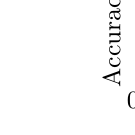
\begin{tikzpicture}
			\path[use as bounding box] (-1.5,0) rectangle (-2.5,1);
			\node[rotate=90] at (-1.40,0.9) {\small Accuracy};

			% \draw[white] (0,0) -- (0, 2);
			\draw[thick, white] (-0.665, 0) -- (0, 0);

			\node at (-0.95, 0.08) {\small \ymin};
			% \node at (-0.95, 0.70) {\small 0.8};
			% \node at (-0.95, 1.24) {\small 0.9};
			\node at (-0.95, 1.7) {\small \ymax};
		\end{tikzpicture}
	} &
	\subfigure {
	  \begin{tikzpicture}
		\path[use as bounding box] (0,0) rectangle (2,1.2);
			\begin{axis}[
				width=0.46\textwidth,
				height=0.28\textwidth,
				cycle list/Paired,
				cycle from colormap manual style,
				ymin=\ymin, ymax=\ymax,
				xmin= 0, xmax= \xmax,
				xmajorticks=false,
				ymajorticks=false,
				xtick pos=left,
				ytick={0.7,0.8,0.9,1},
				yticklabels={0.7,0.8,0.9,1.0},
				xmajorgrids=true,
				ymajorgrids=true,
				axis line style={draw=gray!50, thick},
				]
					\addplot [no marks, very thick, max_prob] table [x={n}, y={max_prob}, col sep=comma] {files/student_port_bin_100_noise_0.0_GeFs_arc.csv};
					\addplot [no marks, very thick, margin] table [x={n}, y={margin_of_confidence}, col sep=comma] {files/student_port_bin_100_noise_0.0_GeFs_arc.csv};
					\addplot [no marks, very thick, total] table [x={n}, y={total}, col sep=comma] {files/student_port_bin_100_noise_0.0_GeFs_arc.csv};
					\addplot [no marks, very thick, aleatoric] table [x={n}, y={aleatoric}, col sep=comma] {files/student_port_bin_100_noise_0.0_GeFs_arc.csv};
					\addplot [no marks, very thick, entropies] table [x={n}, y={entropies}, col sep=comma] {files/student_port_bin_100_noise_0.0_GeFs_arc.csv};
					\addplot [no marks, very thick, epistemic] table [x={n}, y={epistemic}, col sep=comma] {files/student_port_bin_100_noise_0.0_GeFs_arc.csv};
					\addplot [no marks, very thick, epsglob] table [x={n}, y={global_eps}, col sep=comma] {files/student_port_bin_100_noise_0.0_GeFs_arc.csv};
					\addplot [no marks, very thick, epsloc] table [x={n}, y={local_eps}, col sep=comma] {files/student_port_bin_100_noise_0.0_GeFs_arc.csv};


			\end{axis}
				\node[fill=white, opacity=0.6, rounded corners, inner sep=0.1] at (2.55, 0.17) {\scriptsize \(N_{\mathrm{train}}=\NtrainB, \mathrm{DS}=\noiseA\)};
		\end{tikzpicture}
	   } &
	%%%%%%%%%%%%%%%%%%%%%% 5 %%%%%%%%%%%%%%%%%%%%%%%%%%%%%%%%%%%
	\subfigure {
	  \begin{tikzpicture}
		\path[use as bounding box] (0,0) rectangle (2,1.2);
			\begin{axis}[
				width=0.46\textwidth,
				height=0.28\textwidth,
				cycle list/Paired,
				cycle from colormap manual style,
				ymin=\ymin, ymax=\ymax,
				xmin= 0, xmax= \xmax,
				xmajorticks=false,
				ymajorticks=false,
				xtick pos=left,
				xmajorgrids=true,
				ymajorgrids=true,
				axis line style={draw=gray!50, thick},
				]
					\addplot [no marks, very thick, max_prob] table [x={n}, y={max_prob}, col sep=comma] {files/student_port_bin_100_noise_0.1_GeFs_arc.csv};
					\addplot [no marks, very thick, margin] table [x={n}, y={margin_of_confidence}, col sep=comma] {files/student_port_bin_100_noise_0.1_GeFs_arc.csv};
					\addplot [no marks, very thick, total] table [x={n}, y={total}, col sep=comma] {files/student_port_bin_100_noise_0.1_GeFs_arc.csv};
					\addplot [no marks, very thick, aleatoric] table [x={n}, y={aleatoric}, col sep=comma] {files/student_port_bin_100_noise_0.1_GeFs_arc.csv};
					\addplot [no marks, very thick, entropies] table [x={n}, y={entropies}, col sep=comma] {files/student_port_bin_100_noise_0.1_GeFs_arc.csv};
					\addplot [no marks, very thick, epistemic] table [x={n}, y={epistemic}, col sep=comma] {files/student_port_bin_100_noise_0.1_GeFs_arc.csv};
					\addplot [no marks, very thick, epsglob] table [x={n}, y={global_eps}, col sep=comma] {files/student_port_bin_100_noise_0.1_GeFs_arc.csv};
					\addplot [no marks, very thick, epsloc] table [x={n}, y={local_eps}, col sep=comma] {files/student_port_bin_100_noise_0.1_GeFs_arc.csv};


			\end{axis}
				\node[fill=white, opacity=0.6, rounded corners, inner sep=0.1] at (2.55, 0.17) {\scriptsize \(N_{\mathrm{train}}=\NtrainB, \mathrm{DS}=\noiseB\)};
		\end{tikzpicture}
	   } &
	%%%%%%%%%%%%%%%%%%%%%% 6 %%%%%%%%%%%%%%%%%%%%%%%%%%%%%%%%%%%
	\subfigure {
	  \begin{tikzpicture}
		\path[use as bounding box] (0,0) rectangle (2,1.2);
			\begin{axis}[
				width=0.46\textwidth,
				height=0.28\textwidth,
				cycle list/Paired,
				cycle from colormap manual style,
				ymin=\ymin, ymax=\ymax,
				xmin= 0, xmax= \xmax,
				xtick pos=left,
				xmajorticks=false,
				ymajorticks=false,
				xmajorgrids=true,
				ymajorgrids=true,
				axis line style={draw=gray!50, thick},
				]
					\addplot [no marks, very thick, max_prob] table [x={n}, y={max_prob}, col sep=comma] {files/student_port_bin_100_noise_0.2_GeFs_arc.csv};
					\addplot [no marks, very thick, margin] table [x={n}, y={margin_of_confidence}, col sep=comma] {files/student_port_bin_100_noise_0.2_GeFs_arc.csv};
					\addplot [no marks, very thick, total] table [x={n}, y={total}, col sep=comma] {files/student_port_bin_100_noise_0.2_GeFs_arc.csv};
					\addplot [no marks, very thick, aleatoric] table [x={n}, y={aleatoric}, col sep=comma] {files/student_port_bin_100_noise_0.2_GeFs_arc.csv};
					\addplot [no marks, very thick, entropies] table [x={n}, y={entropies}, col sep=comma] {files/student_port_bin_100_noise_0.2_GeFs_arc.csv};
					\addplot [no marks, very thick, epistemic] table [x={n}, y={epistemic}, col sep=comma] {files/student_port_bin_100_noise_0.2_GeFs_arc.csv};
					\addplot [no marks, very thick, epsglob] table [x={n}, y={global_eps}, col sep=comma] {files/student_port_bin_100_noise_0.2_GeFs_arc.csv};
					\addplot [no marks, very thick, epsloc] table [x={n}, y={local_eps}, col sep=comma] {files/student_port_bin_100_noise_0.2_GeFs_arc.csv};


			\end{axis}
				\node[fill=white, opacity=0.6, rounded corners, inner sep=0.1] at (2.55, 0.17) {\scriptsize \(N_{\mathrm{train}}=\NtrainB, \mathrm{DS}=\noiseC\)};
		\end{tikzpicture}
		} \\

	%%%%%%%%%%%%%%%%%%%%%% 7 %%%%%%%%%%%%%%%%%%%%%%%%%%%%%%%%%%%

	\subfigure {
		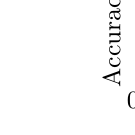
\begin{tikzpicture}
			\path[use as bounding box] (-1.5,0) rectangle (-2.5,1);
			\node[rotate=90] at (-1.40,0.9) {\small Accuracy};

			% \draw[white] (0,0) -- (0, 2);
			\draw[thick, white] (-0.665, 0) -- (0, 0);

			\node at (-0.95, 0.08) {\small \ymin};
			% \node at (-0.95, 0.70) {\small 0.8};
			% \node at (-0.95, 1.24) {\small 0.9};
			\node at (-0.95, 1.7) {\small \ymax};
		\end{tikzpicture}
	} &
	\subfigure {
	  \begin{tikzpicture}
		\path[use as bounding box] (0,0) rectangle (2,1.2);
			\begin{axis}[
				width=0.46\textwidth,
				height=0.28\textwidth,
				cycle list/Paired,
				cycle from colormap manual style,
				ymin=\ymin, ymax=\ymax,
				xmin= 0, xmax= \xmax,
				xtick pos=left,
				xmajorticks=false,
				ymajorticks=false,
				xmajorgrids=true,
				ymajorgrids=true,
				axis line style={draw=gray!50, thick},
				]
					\addplot [no marks, very thick, max_prob] table [x={n}, y={max_prob}, col sep=comma] {files/student_port_bin_50_noise_0.0_GeFs_arc.csv};
					\addplot [no marks, very thick, margin] table [x={n}, y={margin_of_confidence}, col sep=comma] {files/student_port_bin_50_noise_0.0_GeFs_arc.csv};
					\addplot [no marks, very thick, total] table [x={n}, y={total}, col sep=comma] {files/student_port_bin_50_noise_0.0_GeFs_arc.csv};
					\addplot [no marks, very thick, aleatoric] table [x={n}, y={aleatoric}, col sep=comma] {files/student_port_bin_50_noise_0.0_GeFs_arc.csv};
					\addplot [no marks, very thick, entropies] table [x={n}, y={entropies}, col sep=comma] {files/student_port_bin_50_noise_0.0_GeFs_arc.csv};
					\addplot [no marks, very thick, epistemic] table [x={n}, y={epistemic}, col sep=comma] {files/student_port_bin_50_noise_0.0_GeFs_arc.csv};
					\addplot [no marks, very thick, epsglob] table [x={n}, y={global_eps}, col sep=comma] {files/student_port_bin_50_noise_0.0_GeFs_arc.csv};
					\addplot [no marks, very thick, epsloc] table [x={n}, y={local_eps}, col sep=comma] {files/student_port_bin_50_noise_0.0_GeFs_arc.csv};


			\end{axis}
				\node[fill=white, opacity=0.6, rounded corners, inner sep=0.1] at (2.55, 0.17) {\scriptsize \(N_{\mathrm{train}}=\NtrainC, \mathrm{DS}=\noiseA\)};
		\end{tikzpicture}
	} &
	%%%%%%%%%%%%%%%%%%%%%% 8 %%%%%%%%%%%%%%%%%%%%%%%%%%%%%%%%%%%
	\subfigure {
	  \begin{tikzpicture}
		\path[use as bounding box] (0,0) rectangle (2,1.2);
			\begin{axis}[
				width=0.46\textwidth,
				height=0.28\textwidth,
				cycle list/Paired,
				cycle from colormap manual style,
				ymin=\ymin, ymax=\ymax,
				xmin= 0, xmax= \xmax,
				xtick pos=left,
				xmajorticks=false,
				ymajorticks=false,
				xmajorgrids=true,
				ymajorgrids=true,
				axis line style={draw=gray!50, thick},
				]
					\addplot [no marks, very thick, max_prob] table [x={n}, y={max_prob}, col sep=comma] {files/student_port_bin_50_noise_0.1_GeFs_arc.csv};
					\addplot [no marks, very thick, margin] table [x={n}, y={margin_of_confidence}, col sep=comma] {files/student_port_bin_50_noise_0.1_GeFs_arc.csv};
					\addplot [no marks, very thick, total] table [x={n}, y={total}, col sep=comma] {files/student_port_bin_50_noise_0.1_GeFs_arc.csv};
					\addplot [no marks, very thick, aleatoric] table [x={n}, y={aleatoric}, col sep=comma] {files/student_port_bin_50_noise_0.1_GeFs_arc.csv};
					\addplot [no marks, very thick, entropies] table [x={n}, y={entropies}, col sep=comma] {files/student_port_bin_50_noise_0.1_GeFs_arc.csv};
					\addplot [no marks, very thick, epistemic] table [x={n}, y={epistemic}, col sep=comma] {files/student_port_bin_50_noise_0.1_GeFs_arc.csv};
					\addplot [no marks, very thick, epsglob] table [x={n}, y={global_eps}, col sep=comma] {files/student_port_bin_50_noise_0.1_GeFs_arc.csv};
					\addplot [no marks, very thick, epsloc] table [x={n}, y={local_eps}, col sep=comma] {files/student_port_bin_50_noise_0.1_GeFs_arc.csv};


			\end{axis}
				\node[fill=white, opacity=0.6, rounded corners, inner sep=0.1] at (2.55, 0.17) {\scriptsize \(N_{\mathrm{train}}=\NtrainC, \mathrm{DS}=\noiseB\)};
		\end{tikzpicture}
	} &
	%%%%%%%%%%%%%%%%%%%%%% 9 %%%%%%%%%%%%%%%%%%%%%%%%%%%%%%%%%%%
	\subfigure {
	  \begin{tikzpicture}
		\path[use as bounding box] (0,0) rectangle (2,1.2);
			\begin{axis}[
				width=0.46\textwidth,
				height=0.28\textwidth,
				cycle list/Paired,
				cycle from colormap manual style,
				ymin=\ymin, ymax=\ymax,
				xmin= 0, xmax= \xmax,
				xtick pos=left,
				xmajorticks=false,
				ymajorticks=false,
				xmajorgrids=true,
				ymajorgrids=true,
				axis line style={draw=gray!50, thick},
				]
					\addplot [no marks, very thick, max_prob] table [x={n}, y={max_prob}, col sep=comma] {files/student_port_bin_50_noise_0.2_GeFs_arc.csv};
					\addplot [no marks, very thick, margin] table [x={n}, y={margin_of_confidence}, col sep=comma] {files/student_port_bin_50_noise_0.2_GeFs_arc.csv};
					\addplot [no marks, very thick, total] table [x={n}, y={total}, col sep=comma] {files/student_port_bin_50_noise_0.2_GeFs_arc.csv};
					\addplot [no marks, very thick, aleatoric] table [x={n}, y={aleatoric}, col sep=comma] {files/student_port_bin_50_noise_0.2_GeFs_arc.csv};
					\addplot [no marks, very thick, entropies] table [x={n}, y={entropies}, col sep=comma] {files/student_port_bin_50_noise_0.2_GeFs_arc.csv};
					\addplot [no marks, very thick, epistemic] table [x={n}, y={epistemic}, col sep=comma] {files/student_port_bin_50_noise_0.2_GeFs_arc.csv};
					\addplot [no marks, very thick, epsglob] table [x={n}, y={global_eps}, col sep=comma] {files/student_port_bin_50_noise_0.2_GeFs_arc.csv};
					\addplot [no marks, very thick, epsloc] table [x={n}, y={local_eps}, col sep=comma] {files/student_port_bin_50_noise_0.2_GeFs_arc.csv};


			\end{axis}
				\node[fill=white, opacity=0.6, rounded corners, inner sep=0.1] at (2.55, 0.17) {\scriptsize \(N_{\mathrm{train}}=\NtrainC, \mathrm{DS}=\noiseC\)};
		\end{tikzpicture}
	} \\

	%%%%%%%%%%%%%%%%%%%%%% 10 %%%%%%%%%%%%%%%%%%%%%%%%%%%%%%%%%%%
	\subfigure {
	} &

	\subfigure {
		
\begin{tikzpicture}
			\path[use as bounding box] (0,-0.5) rectangle (2,-1.6);
			\node at (1.975,-0.25) {\small Acceptance rate};
			\node at (0.1, 0.15) {\small 0};
			\node at (0.8, 0.15) {\small 0.2};
			\node at (1.6, 0.15) {\small 0.4};
			\node at (2.4, 0.15) {\small 0.6};
			\node at (3.2, 0.15) {\small 0.8};
			\node at (3.95, 0.15) {\small 1};
		\end{tikzpicture}
	} &
	\subfigure {
		
\begin{tikzpicture}
			\path[use as bounding box] (0,-0.5) rectangle (2,-1.6);
			\node at (1.975,-0.25) {\small Acceptance rate};
			\node at (0.1, 0.15) {\small 0};
			\node at (0.8, 0.15) {\small 0.2};
			\node at (1.6, 0.15) {\small 0.4};
			\node at (2.4, 0.15) {\small 0.6};
			\node at (3.2, 0.15) {\small 0.8};
			\node at (3.95, 0.15) {\small 1};
		\end{tikzpicture}
	} &
	\subfigure {
		
\begin{tikzpicture}
			\path[use as bounding box] (0,-0.5) rectangle (2,-1.6);
			\node at (1.975,-0.25) {\small Acceptance rate};
			\node at (0.1, 0.15) {\small 0};
			\node at (0.8, 0.15) {\small 0.2};
			\node at (1.6, 0.15) {\small 0.4};
			\node at (2.4, 0.15) {\small 0.6};
			\node at (3.2, 0.15) {\small 0.8};
			\node at (3.95, 0.15) {\small 1};
		\end{tikzpicture}
	} \\
	\end{tabular}
\end{figure}

\end{document}